% \chapter{Spin states of the Dirac cone}
\section{Spin states of the Dirac cone}
Similar to the discussion in \cref{sec:spin-orbit} on the spin structure of a system with Rashba coupling, we here consider the spin structure of the Weyl cone.
We begin by finding the eigenstates of the Weyl Hamlitonian \( H = v_F \vec{\sigma} \vec{p} \).
Assume plane wave states, and some arbitrary linear combination of spin up and spin down,
\[
  \psi _{\pm} = e^{i \vec{k} \vec{r}} \alpha
  \begin{pmatrix}
    1\\
    b
  \end{pmatrix},
\]
where \(\alpha \) is some normalization.
Solving the time independent Schrodinger equation
\[
H \psi = E \psi,
\]
we find
\begin{equation}
  \label{eq:132}
  b = -\frac{k_{z} \pm k}{k_{x} - i k_{y}}.
\end{equation}
Requiring normalized states \(\braket{\psi | \psi } = 1\) gives the normalization
\[
|\alpha |^2 = \frac{1}{1 + |b|^2}.
\]

Having found the states, we find the spin expectation value
\begin{equation}
  \label{eq:133}
  \vec{S} = \braket{\psi | \hat{S} | \psi },
\end{equation}
where \(\vec{S}\) is the spin expectation value and \(\hat{S} = \frac{\vec{\sigma}}{2} \) is the spin operator, where \(\hbar \) was set to 1.
Simply evaluating \cref{eq:133}, yields
\begin{equation}
  \label{eq:134}
  \vec{S} = \pm \frac{\vec{k}}{2 k}.
\end{equation}

The spin structure is that of a hedgehog.

\begin{figure}[ht]
  \centering
  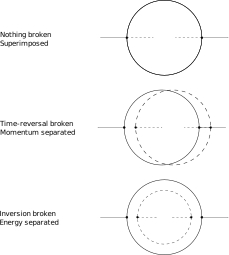
\includegraphics[width=0.75\textwidth]{figures/spinStructureWeyl}
  \caption{\label{fig:spinStructure} }
\end{figure}
